% Initialisation
\documentclass[
	fontsize=11pt
	headlines=2,
	footlines=2,
	parskip=half
]{scrartcl}

\usepackage[left=2.54cm,top=2.54cm,right=2.54cm,bottom=2.54cm,headheight=30pt]{geometry}

% Enforce UTF8 encoding
\usepackage[utf8]{inputenc}

% Colours
\usepackage[dvipsnames]{xcolor}

% Header and footer
\usepackage{scrlayer-scrpage}
\ohead{SENG4800A - Individual interim report \\ \today}
\cfoot{\pagemark}

% Document title and author
\title{Exploring 3D Geovisualisation Techniques and their Applications with Large Datasets using HTML5 and WebGL}
\author{Monica Olejniczak}

% Sections
\usepackage[compact]{titlesec}

% http://tex.stackexchange.com/questions/198830/section-title-with-runin-and-koma-class

% Abstract
\usepackage{abstract}
\setlength{\absleftindent}{0pt}
\setlength{\absrightindent}{0pt}
\renewcommand{\absnamepos}{flushleft}
\renewcommand{\abstractnamefont}{\normalfont\Large\bfseries}

% Links
\usepackage{hyperref}

% Todo notes
\usepackage{todonotes}
\presetkeys{todonotes}{inline}{}

% Gantt charts
\usepackage{pgfgantt}

% Tables
\usepackage{booktabs}
\usepackage{tabularx}
\renewcommand{\arraystretch}{1.5}
\setlength{\textfloatsep}{0.1em}

% Figures
\usepackage{wrapfig}
\usepackage{caption}
\usepackage[font=scriptsize]{subcaption}

\newcommand{\subfigcaptionskip}{\vspace{-10pt}}

% Remove spacing before and after captions
\captionsetup[table]{aboveskip=-8pt}
\captionsetup[table]{belowskip=8pt}
\captionsetup[figure]{belowskip=-10pt}

% Additional
\usepackage{float}
\usepackage{spreadtab}
\usepackage{etoolbox}

% References
\usepackage[backend=bibtex,style=authoryear]{biblatex}
\addbibresource{references.bib}
\renewcommand*{\bibfont}{\small}
\DeclareBibliographyCategory{exclude}
\newcommand{\bibentry}[1]{
	\addtocategory{exclude}{#1}
	\fullcite{#1}
}

% Appendices
\usepackage[toc,page]{appendix}

% Commands
\newcommand{\rating}[1]{
	\ifnumless{#1}{20 * 100} {Very low} {
		\ifnumless{#1}{40 * 100} {Low} {
			\ifnumless{#1}{60 * 100} {Medium} {
				\ifnumless{#1}{80 * 100} {High} {
					Very high
				}
           	}
		}
	}
}

\begin{document}

	% Title
	\makeatletter
		\textbf{\LARGE\textsf{\@title}}
		\vspace{-2.5em}
		\begin{center}
			\large\textbf{\textsf{\@author}}
		\end{center}
		\vspace{-2.5em}
	\makeatother

	\begin{abstract}
		Lorem ipsum dolor sit amet, consectetur adipiscing elit. Quisque nec felis vel ipsum scelerisque interdum. Duis velit magna, efficitur vitae tortor vitae, efficitur lacinia ligula. Praesent euismod ut nulla fringilla porttitor. Maecenas sit amet libero ut magna pellentesque tristique sed in nibh. Integer quis interdum nibh. Nam suscipit malesuada mi quis porttitor. Sed sed tristique mi. Aliquam arcu est, lobortis nec sodales ut, facilisis ac lorem. In hac habitasse platea dictumst. Vivamus et elementum libero, eu hendrerit enim. Mauris blandit dui vitae elit pulvinar mollis. Curabitur sollicitudin scelerisque est. Nunc imperdiet felis quis lectus scelerisque convallis. Maecenas et erat nec odio cursus euismod eu ut lacus.

		Mauris libero turpis, imperdiet et odio et, condimentum tincidunt massa. Nunc nec nulla eu mauris maximus varius. Quisque condimentum porta nisi, sit amet maximus quam bibendum sed. Sed placerat maximus ligula, in dignissim ex consequat a. Proin consequat, neque non fringilla imperdiet, sem orci.
	\end{abstract}
	
	\section{Introduction} {
	\label{sec:introduction}

		Geovisualisation is the interactive visualisation of geospatial information, which is closely related to the fields of scientific and information visualisation \parencite{jiang2005geovisualization}. Geovisualisations are particularly important in data analytics and when working with large datasets, since they enable data exploration and decision-making processes when combined with human understanding \parencite{grinstein2002introduction, hendley1995case}. This is due to the addition of the geographical dimension in the visualisation process, which greatly facilitates the identification and interpretation of spatial patterns and relationships in complex data \parencite{kwan2004geovisualization}.

		This project will attempt to 

		% This project will attempt to improve student learning by aiding teachers with real-time feedback using mobile visual analytics. Multi-touch tablet devices can be carried by a teacher in a classroom environment, and provide a portable, intuitive and familiar interface to display analytics regarding student learning.
		
		This report explores 3D geovisualisation techniques, discusses the World Wide Web as a platform for geovisualisations and common interactions found in 3D geovisualisations. Next, the applications of geovisualisations are analysed and an overview of the project is provided from this research. Then, the aims and details of this project are discussed which include its goals, plan for development and schedule. Finally, this report concludes with the ethical issues that arise from developing this project.

		\subsection{3D geovisualisation techniques} {

			\textcite{bleisch2012geovisualization} defines two distinct categories that represent most 3D geovisualisations: 3D representations of the real world and a combination of 3D representations of the real world with abstract data.

			The \emph{3D representations of the real world} category represents the real world and its objects in realistic or generalised ways to communicate information. This category often uses x, y and z coordinates to show the real world dimensions \textendash\, easting, northing, elevation and sometimes the height of buildings or other objects. A 3D environment attempting to represent the real world usually consists of a digital elevation or surface model with either high resolution orthoimagery, satellite imagery or maps \parencite{bleisch2012geovisualization}.

			\newcommand{\combinationwidth}{0.45\textwidth}
			\begin{wrapfigure}{r}{\combinationwidth}
				\centering
				\captionsetup{font=small}
                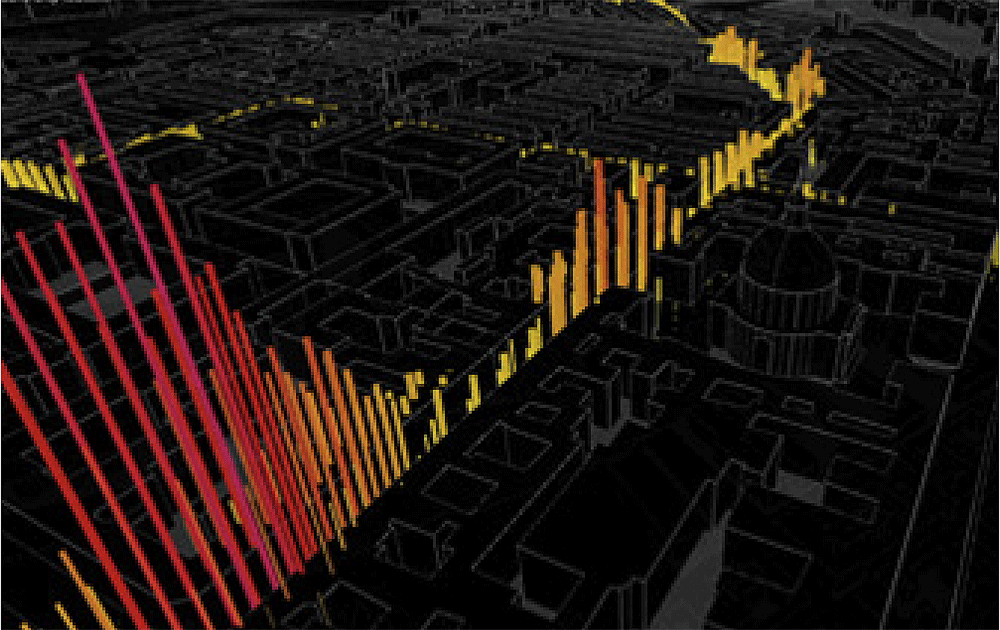
\includegraphics[width=\combinationwidth]{images/category-combination}
				\caption{An example of combining 3D representations of the real world with abstract data. \protect\footnotemark}
				\label{fig:category_combination}
				\vspace{-5pt}
			\end{wrapfigure}

			\footnotetext{\bibentry{ratti2010copenhagen}}

			Common examples of this category are digital city models and virtual globes. 3D city models often apply photo texturing to suggest additional detail, since the detail may not be present in the underlying geometric model of the city \parencite{bleisch2012geovisualization}.

			In the \emph{combination of 3D representations of the real world with abstract data} category, the representation of the real world environment is enhanced with the inclusion of data displays. This category is designed for communicating, analysing and explorating data and depicts the real world dimensions and data values through the x, y and z axes. An example of this category is shown in Figure~\ref{fig:category_combination} \parencite{bleisch2012geovisualization}.

			To visualise the data displays in this category, triangle meshes, texture maps or non-uniform rational B-spline (NURBS) surfaces can be created and applied to the visualisation. NURBS in particular are computationally efficient and effective at modelling complex structures \parencite{hildebrandt2011image, zhong2006enhanced}.

		}

		\subsection{Geovisualisations using the World Wide Web} {

			Geovisualisations can be realised through the World Wide Web, which has become a prominent medium for publishing geospatial data. The web facilitates the creation of immersive and highly interactive environments, which can be taken advantage of to explore and present dynamic geospatial data \parencite{maceachren2001research}.

			WebGL is a cross-platform web standard for a 3D graphics API derived from OpenGL, which has been exposed through the HTML5 canvas element \parencite{marrin2011webgl} as a drawing context. It is widely supported in modern browsers, without needing additional plug-ins or extensions, and is designed for building dynamic applications that require 3D visualisations \parencite{chaturvedi2015web, marrin2011webgl, parisi2012webgl}. Rendering such visualisations in real-time is possible due to the accelerated graphics rendering provided by WebGL, which utilises the graphics card memory on a device \parencite{chaturvedi2015web} to perform multiple operations in parallel to one another.

		}

		\subsection{Interaction in geovisualisations} {

			The communication between a user and a system, otherwise known as \emph{interaction}, is an important aspect in geovisualisation. Interaction enables users to explore the data presented to them in order to uncover trends and allow for decision-making processes \parencite{yi2007toward}. It is also essential for visualisations to support interaction, otherwise the usefulness of the visualisation is greatly limited as the dataset that it represents grows larger \parencite{yi2007toward}.

			In the context of geovisualisation, the user should be able to navigate the visualisation itself and the synthetic geography that it represents. Navigation enables particular and pertinent information to be located more successfully and is considered to be one of the most important metaphors for dynamic cartography \parencite{cartwright2001geospatial}. The navigation of a geospatial representation requires the user to perform standard operations, which include: translate, scale, rotate, map projection, manipulation of the design representation parameters, level of generalisation and field of view \parencite{cartwright2001geospatial, hand1997survey}.

		}

		\subsection{Applications of geovisualisation} {

			% equipped assist

			There is a comprehensive amount of geospatial data available, which has been made accessible through various digital data resources. Census enumerations, health statistics, land use categories, meteorological measurements, telephone information and transportation records constitute examples of geospatially referenced data that can be applied to geovisualisations for scientific, research and societal purposes. Furthermore, this widely accessible geospatial data has resulted in an equally large range of application domains for geovisualisations, which include earth science, public health and social science as shown in Figure~\ref{fig:geovisualisation_applications} \parencite{maceachren2004geovisualization}.

			\newcommand{\applicationwidth}{0.32\textwidth}
			\newcommand{\applicationheight}{3cm}
			\begin{figure}[H]
				\centering
		        \begin{subfigure}[b]{\applicationwidth}
	                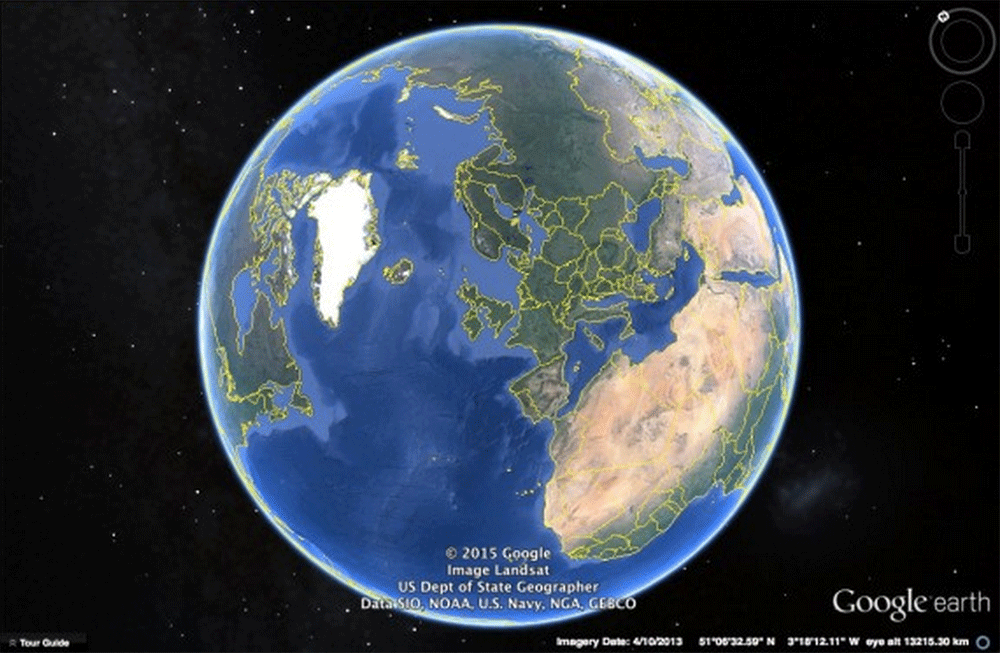
\includegraphics[width=\textwidth,height=\applicationheight]{images/earth-science}
	                \caption{Earth science \parencite{google2015earth}}
	                % \protect\footnotemark}
	                \label{fig:earth_science}
		        \end{subfigure}
		        \begin{subfigure}[b]{\applicationwidth}
	                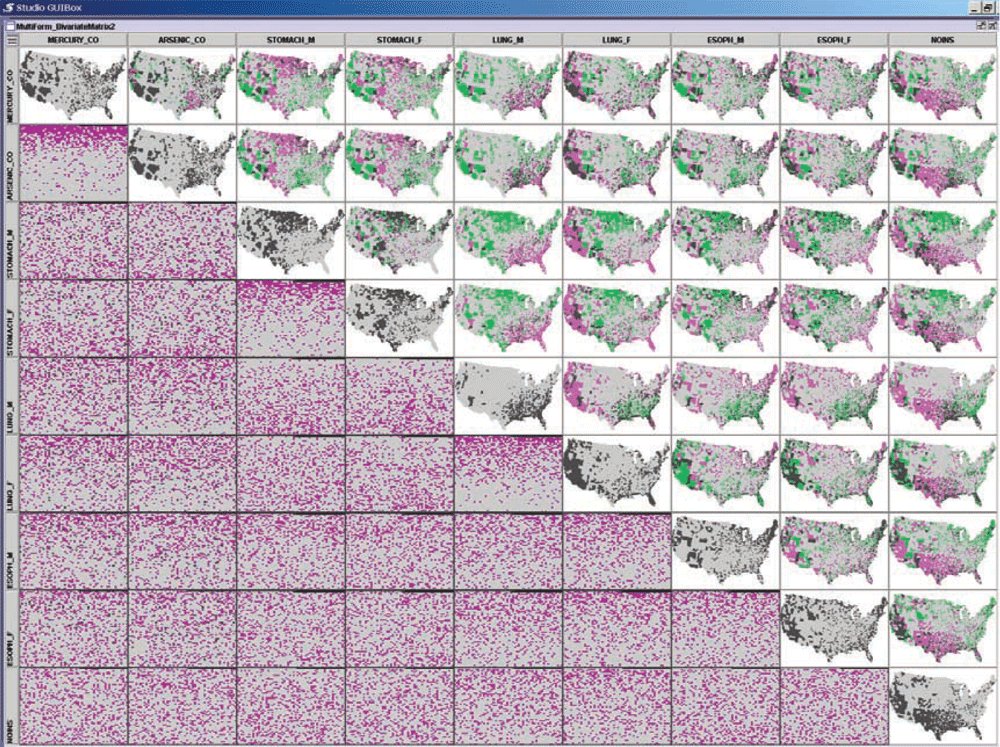
\includegraphics[width=\textwidth,height=\applicationheight]{images/public-health}
	                	\caption{\tiny{Public health \parencite{maceachren2004geovisualization}}}
	                \label{fig:public_health}
		        \end{subfigure}
		        \begin{subfigure}[b]{\applicationwidth}
	                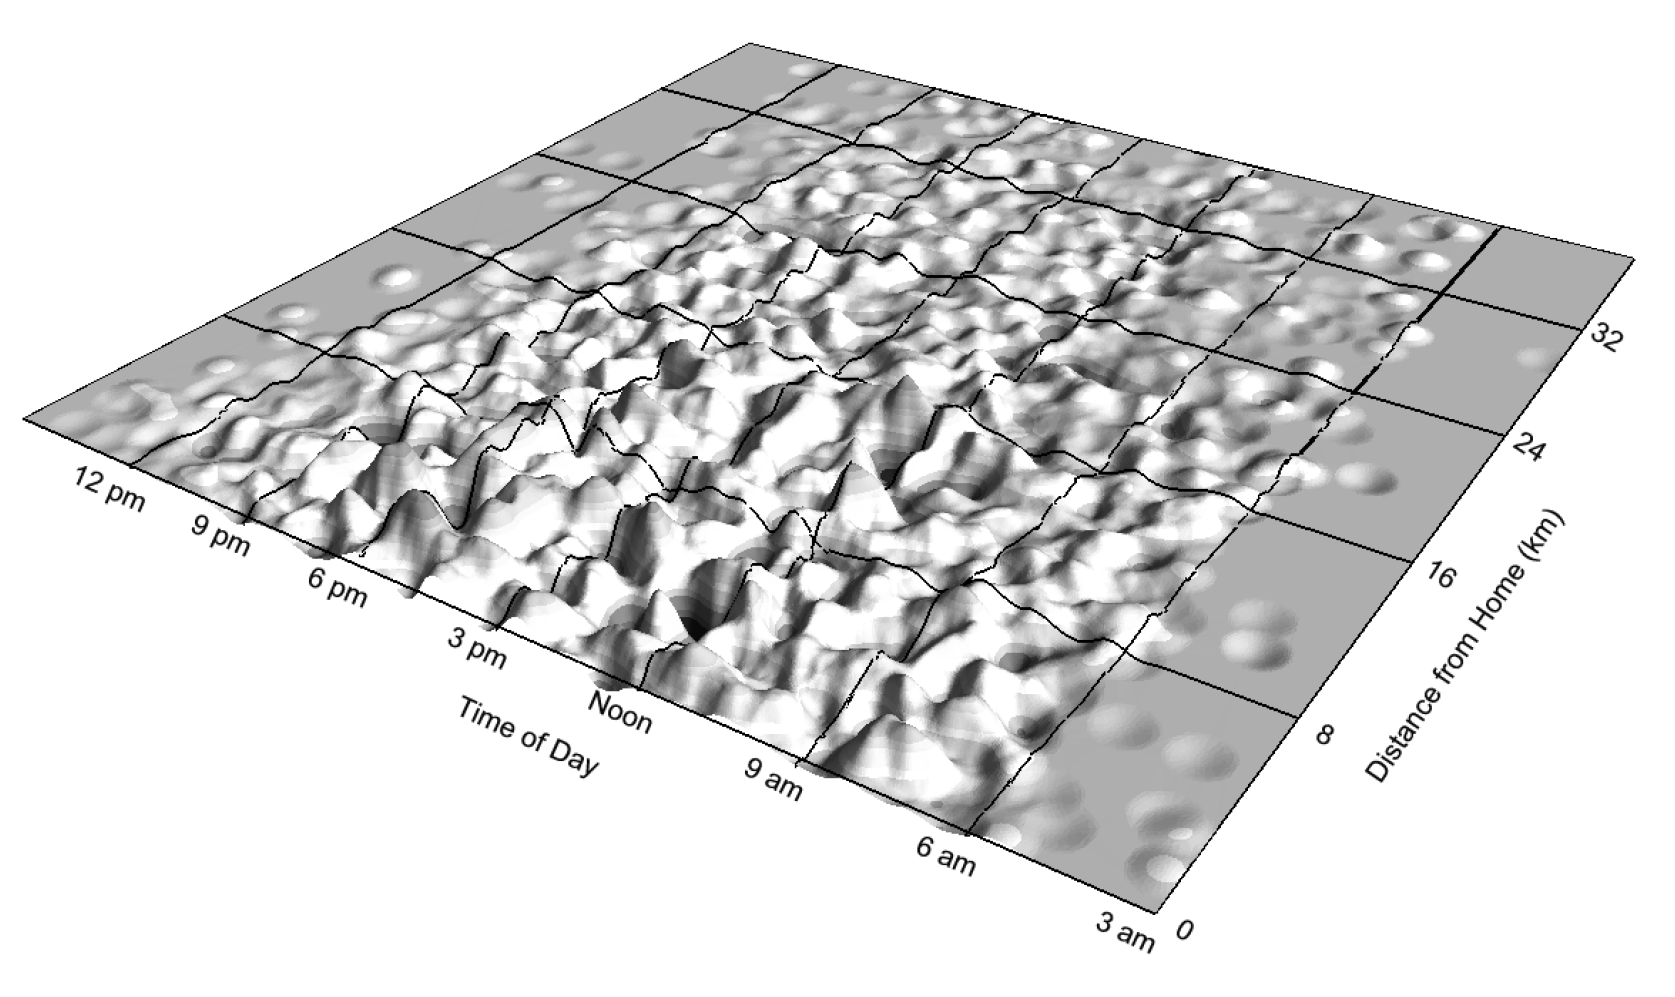
\includegraphics[width=\textwidth,height=\applicationheight]{images/social-science}
	                	\caption{Social science \parencite{kwan2004geovisualization}}
	                \label{fig:social_science}
		        \end{subfigure}
				\caption{Application domains for geovisualisation.}
				\subfigcaptionskip
				\label{fig:geovisualisation_applications}
			\end{figure}

			% \footnotetext{\bibentry{google2015earth}}

			% Earth science
			In the domain of \emph{earth science}, the visualisation of environmental data reveals new insights into the patterns of nature and human-related phenomena. These visualisations also help improve the understanding of the dynamic processes of earth systems \parencite{yu2012google}.

			\textcite{yu2012google} analyses virtual globes as a tool in earth science applications, which have been developed to effectively facilitate data collection, exploration and the visualisation of environmental data. They deliver huge volumes of satellite imagery, 3D views of the earth, topographic maps and distance measurement to the general public. These globes have promoted entertainment, education, the exploration of new findings, data sharing and provided researchers with effective channels of communicating their findings. Virtual globes can be applied to many areas and in the case of \emph{Google Earth}, typically focus on large-scale phenomena in the atmosphere, carbon science, ecosystems, energy, geology and natural disasters.

			% Public health
			Within \emph{public health}, geovisualisations can be modelled to geospatial data concerning risk factors, health outcomes and interventions to provide an opportunity to understand and act on the varied geographic distribution of disease. However, these datasets are typically difficult to analyse through traditional methods as the data is highly multivariate \parencite{maceachren2004geovisualization}.

			\textcite{maceachren2004geovisualization} were able to apply a mortality and risk factor dataset to a geovisualisation, in order to explore the spatial and nonspatial relationships in this data. They considered environmental risk factors, health care access and cancer mortality rates of various ages and genders to demonstrate that it is possible to utilise geovisualisations in a way that addresses critical issues in public health.

			% Social science
			An important research area in \emph{social science} is the study of human activities and movements in space and time. Geovisualisations can model this data, which has become feasible with the increased availability of georeferenced individual-level data \parencite{kwan2004geovisualization}.

			\textcite{kwan2004geovisualization} studied gender and ethnic differences in space-time activity patterns in a metropolitan area. Their study demonstrated that geovisualisation methods are effective in revealing the complex interaction between the spatial and temporal dimensions in structuring human spatial behaviour. \citeauthor{kwan2004geovisualization} also discovered that geovisualisation tools can help formulate more realistic computational or behavioural models for exploratory spatial data analysis.

		}

		% \subsection{Challenges and issues} {

		% 	\todo{geospatial info visualisation -
		% 	geoagents - Can geovisualization products offer too much information? The Web enables access to vast stores of information,
		% 	much of it with geospatial referencing, thus Web-based geovisualization has the potential to
		% 	overwhelm users with a huge volume of unorganized information. The key question here is how can we
		% 	provide the “information filters” that avoid this overload and allow users to work with a myriad of information.}

		% }

		\subsection{Overview} {

			In this work, HTML5 and WebGL will be utilised to visualise geographical data, with triangle based meshes and NURBS surface data displays. This ensures the development of a cross-platform system capable of rendering complex visualisations through accelerated graphics rendering. This project will consider several navigation interaction techniques, particularly translation, scaling and rotation. Finally, the visualisations will be applied to both earth and social science datasets as both domains have a wide array of applications.

		}
	
	}
	
	\section{Project plan} {
	\label{sec:project_plan}
		
		This project will be developed in a web environment to ensure the creation of a platform independent system. It will primarily use Three.js~\footnote{\bibentry{cabello2010three}}, a JavaScript library that abstracts WebGL, as a tool for creating 3D visualisations. An initial prototype was designed and has been discussed in Appendix~\ref{app:current_progress}. The main \emph{goals} of this project are to:

		\begin{itemize}
			\item Visualise a large dataset in a time efficient manner.
			% \item Ensure the visualisation is aesthetically pleasing and useful to the user.
			% 	\begin{itemize}
			% 		\item Users should be able to understand and interpret the data without training.
			% 	\end{itemize}
			\item Create visualisations that can be applied to multiple datasets.
			\item Integrate the results into the teaching analytics component of the group project.
			\item Explore how 3D visualisations can effectively convey information.
			\item Apply the visualisations to real datasets and ensure they are scalable.
			\item Explore how to optimise calls and understand what drains processing resources easily.
			\begin{itemize}
				\item This can be measured with a JavaScript performance testing environment~\footnote{\bibentry{bynens2011jsperf}}.
			\end{itemize}
		\end{itemize}
		
		To facilitate these goals, this project will involve creating visualisations that can be: applied to a range of datasets and compared to one another. This will require applying the same datasets to both visualisations and analysing the differences in performance and scalability. With this in mind, it has been decided that heat maps will be used as the basis of this project as they have a wide array of applications. Figure~\ref{fig:heat_maps} features two different ways of visualising a heat map. It has potential applications in displaying a 3D column or bar chart, financial and geographical data. It is interesting to note that geographical data can be applied to both visualisations, where the image on the left can be mapped to a sphere and could represent population data, while the other could represent pollution levels in a city.
		
		\newcommand{\heatmapwidth}{0.4\textwidth}
		\newcommand{\heatmapheight}{3.5cm}
		\begin{figure}[H]
			\centering
			\begin{subfigure}[b]{\heatmapwidth}
                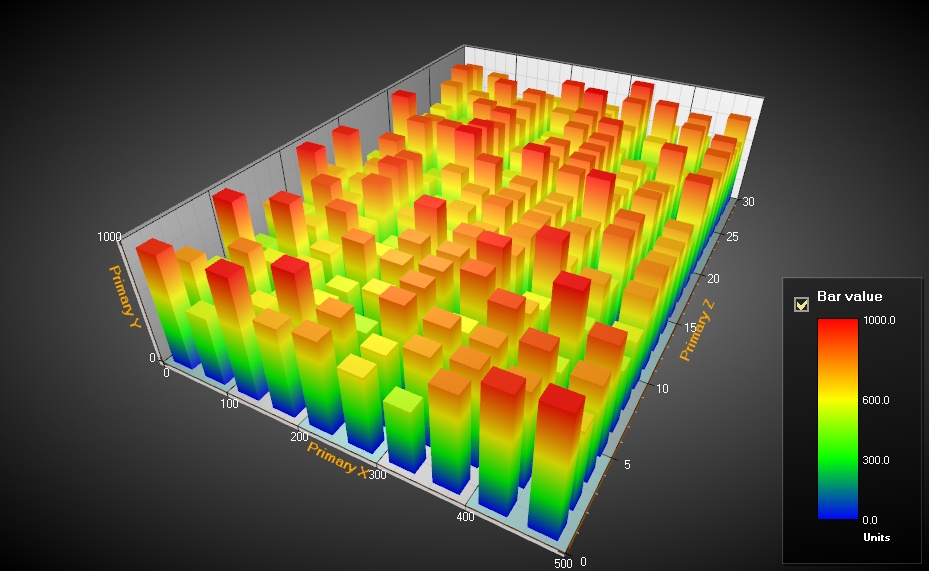
\includegraphics[width=\textwidth,height=\heatmapheight]{images/heat-map-1}
                \caption{Financial data. \protect\footnotemark}
                \label{fig:heat_map_financial}
	        \end{subfigure}
	        \begin{subfigure}[b]{\heatmapwidth}
                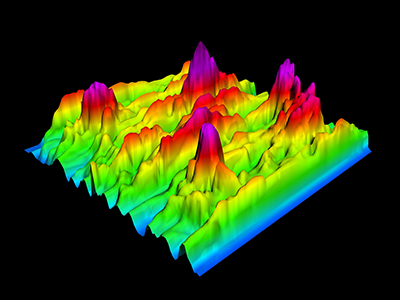
\includegraphics[width=\textwidth,height=\heatmapheight]{images/heat-map-2}
                \caption{Electroencephalogram. \protect\footnotemark}
                \label{fig:heat_map_eeg}
	        \end{subfigure}
			\caption{Two different representations of a heat map.}
			\subfigcaptionskip
			\label{fig:heat_maps}
		\end{figure}

		\footnotetext[5]{\bibentry{tuomainen2014financial}}
		\footnotetext{\bibentry{fuchs2006physiological}}
		
		The data for the visualisations can easily be represented as a flat array and may need to be preprocessed, which depends on the format of the data. This data representation has also been adopted by The WebGL Globe Chrome Experiment~\footnote{\bibentry{google2011globe}}, as shown in Appendix~\ref{app:globe}, is a great example of visualising a large dataset in an efficient way. This open platform project clearly demonstrates that the goals of this project are achievable. They encourage users to use their own datasets, ensuring a certain level of scalability and applications with geographical data.
		
		The development of these visualisations will involve using the established \href{http://threejs.org/docs/#Reference/Extras.Geometries/BoxGeometry}{BoxGeometry} and NURBS surface that are available in Three.js. The \href{http://threejs.org/examples/webgl_geometry_nurbs.html}{NURBS example}, as displayed in Appendix~\ref{app:nurbs}, proves that it is possible to render a smooth 3D surface. This can be applied to represent a heat map and if there lie difficulties in implementing this, then a simpler representation can be modelled.

		\subsection{Deliverables} {
		\label{sec:deliverables}

			The key deliverables of this project have been split into three categories: basic, intermediate and advanced.

			The \emph{basic deliverables} entail developing the implementation for a single visualisation, which should resemble Figure~\ref{fig:heat_map_financial}, with a small, generated dataset. This visualisation will have interactions for panning, zooming and rotating enabling users to navigate the scene.

			The \emph{intermediate deliverables} are concerned with providing users with the ability to filter data, so they are able hide particular information shown on the visualisation. This set of deliverables will also see the implementation of another visualisation, similar to Figure~\ref{fig:heat_map_eeg}, which will initially be applied to a large, generated dataset. The final stage of these deliverables involves applying real datasets, as outlined in Section~\ref{sec:dataset}, to both visualisations.

			The core \emph{advanced deliverables} requires integrating both prototypal visualisations into the group project. Other deliverables include analysing the scalability and computational power to render both visualisations, performing a user study to measure the usefulness of the visualisations and incorporating multi-touch gestures such as pan, pinch, zoom and rotate.

		}

		\subsection{Dataset} {
		\label{sec:dataset}

			As discussed in Section~\ref{sec:deliverables}, the visualisations will begin with generated data so development can begin immediately. Using generated data brings control over the size of the dataset applied to a prototype and enables the scalability of each visualisation can be tested. 

			Following the use of fake data, each prototype will have real datasets applied to them. By using the same data for both prototypes, their differences in computational requirements and scalability can be compared and analysed. GeoNames \footnote{\bibentry{wick2005geonames}} is a geographical database that stores population data for a significant number of cities and their respective latitude and longitude coordinates. This database falls under a creative commons attribution license and will be used for both visualisations because there are no copyright concerns or immediate issues when reading and parsing the data it provides. However, some unnecessary information contained in a GeoNames dataset (such as \emph{geonameid}, \emph{feature class} and  \emph{dem}) will need to be removed. The format of the data should also be modified (from a tab separated list to a JavaScript array) when used with a prototype. These steps are necessary so the visualisations can read the data efficiently and hence reduce the loading time for the user. Other datasets can be obtained from Earthdata~\footnote{\bibentry{nasa2000data}}, but will require further investigation regarding how to extract the information from the available databases.

			Once real data has been applied to both prototypes, the visualisations will be integrated into a live system for the teaching analytics component of the final year project. The amount of touch gestures that particular system components receive and the progress made by students, groups and tutorials will need to be collected and stored in the database. This data can be visualised to aid teachers in analysing ongoing student progress.
		
		}

		\subsection{Evaluation} {
		\label{sec:evaluation}

			The following criteria will be considered when evaluating and comparing the visualisations: time to render, time to perform operations after render, average frames per second, scaling betwen small and large datasets and how different colours and schemes effect performance.

		}

		\subsection{Software development process} {
		\label{sec:software_development_process}

			A rapid application development (RAD) approach will be undertaken when developing this project. This methodology focuses on iterative development and the rapid construction of prototypes, instead of investing significant amounts of time into planning. RAD enables the software to be written quickly through the reuse of software components and engaging in less formal reviews. This process also performs unit, integration and system testing at the end of each construction phase. 

			In this project, each visualisation can be thought of as a single prototype, where parts of the first prototype can be reused for the second visualisation. Testing should be performed during the course of the project, but particularly when a major component of a prototype has been developed, such as data filtering.

		}
		
		\subsection{Development environment} {
		\label{sec:development_environment}

			The tools and libraries that will be used for the development environment of this project have been outlined in Table~\ref{tab:dependencies}. Each technology has been chosen due to the fact that they are popular, easy to use, well documented, maintained and have been used in the past.
		
			\begin{table}[H]
			\caption{The list of project dependencies for the development environment.}
			\label{tab:dependencies}
			\begin{tabularx}{\textwidth}{@{}XX@{}}
				\toprule
				\textbf{Dependency} & \textbf{Description} \\
				\midrule
				Git & Version control \\
				BitBucket & Source code host \\
				SourceTree & Git client \\
				Node.js & Runtime environment \\
				Three.js & WebGL abstraction library \\
				RequireJS & Dependency injection library \\
				Intern & Test runner \\
				Chai & Assertion library \\
				\bottomrule
			\end{tabularx}
			\end{table}
		
		}

		\subsection{Non-functional requirements} {

			The following non-functional requirements are considered key to the success of this project:

			\begin{description}
				\item[Modularity:] The project should be highly modular, so parts of the system can be reused and easily integrated into the group project.
				\item[Performance:] The response time of the system is a major concern when working with a large dataset. The time to load the visualisation is highly dependent on the size of the dataset, graphical processing, network bandwidth and latency. However, once the visualisation has loaded, the user should be faced with near immediate response times (\textless 1 second).
				\item[Scalability:] This is important when modifying the size of the dataset used with a visualisation. The visualisation should be capable of handling increased processing with a larger dataset. Not only this, but the information should remain mapped to the correct locations in the scene with increased volumes of data.
				\item[Testability:] Highly testable code is important when writing test suites, so all aspects of the system can be easily tested to locate faults. In JavaScript:
					\begin{itemize}
						\item A common technique is to hide variables through the use of closure, which leads to untestable code. These variables should be replaced with public variables that are prefixed with an underscore, to indicate they are not a part of the public API.
						\item Anonymous functions should be replaced with named functions so they can be tested.
						\item Dependency injection should be used through RequireJS, so all dependencies can be mocked.
					\end{itemize}
			\end{description}

		}
		
		\subsection{Risks} {
		\label{sec:risks}

			The following table outlines the risks associated with this project. A more detailed risk assessment can be found in Appendix~\ref{app:risk_assessment}.
			
			\begin{table}[H]
			\caption{The list of risks associated with this project and their appropriate mitigation strategies.}
			\begin{tabularx}{\textwidth}{@{}lp{0.35\linewidth}X@{}}
				\toprule
				\textbf{Id} & \textbf{Description} & \textbf{Strategy} \\
				\midrule
				1 & Deliverables are not completed by the deadline. & \emph{Reduction:} Adhere to the project schedule. \\
				2 & Hardware failure. & \emph{Reduction:} Hardware will be treated with care. \\
				3 & Hardware and software cannot efficiently process the visualisation. & \emph{Reduction:} Make optimisations where possible. \\
				4 & Scope is too large. & \emph{Reduction:} Reasonable requirements are established in the proposal with the project supervisor. \\
				5 & Code is lost. & \emph{Reduction:} Version control is used with small commits to minimise the impact of loss. \\
				6 & Project cannot be integrated to the group project. & \emph{Reduction:} Allocate enough time to this and contribute to the group through other means. \\
				7 & Project is not useful or applicable to the group. & \emph{Reduction and acceptance} Discuss and confirm applicability with the group and project supervisor before commencing. Alter the visualisation when required. \\
				\bottomrule
			\end{tabularx}
			\end{table}
		
		}
	
	}
	
	\section{Project schedule} {
	\label{sec:project_schedule}
	
		The project plan, which was outlined in Section~\ref{sec:project_plan}, is to be completed according to the project schedule. Unfortunately, it is quite probable that no work will be undertaken towards the individual project during the mid-year recess. This is due to the need to prepare for and attend RoboCup 2015, China. It has therefore been omitted from the schedule, which has been demonstrated through the Gantt chart in Figure~\ref{fig:schedule}.

		\begin{figure}[H]
	        \makebox[\textwidth][c]{\resizebox{0.95\paperwidth}{!}{\begin{ganttchart}[
	vgrid={*6{black, dotted},*1{black, dashed}},
	x unit=0.3cm,
	y unit title=0.75cm,
	y unit chart=1cm,
	time slot format=isodate,
	title height = 1,
	title/.append style={draw=none, fill=RoyalBlue!40!black},
	title label font=\sffamily\bfseries\color{white},
	title label node/.append style={below=-1.6ex},
	title left shift=.05,
	title right shift=-.05,
	title top shift=.05,
	title height=.95,
	bar/.append style={draw=none, fill=MidnightBlue!75},
	bar height=.6,
	bar label font=\normalsize\color{black!80},
%	group right shift=0,
%	group top shift=.6,
%	group height=.3,
%	group peaks height=.2,
%	bar incomplete/.append style={fill=red}
]
{2015-07-27}{2015-11-08} % start and end date

\newganttchartelement{optionalbar}{
	optionalbar/.style={
		shape=rectangle,
		fill=black!70
	},
	optionalbar height=.6
}

\gantttitle{Semester 2}{105} \ganttnewline
\gantttitlecalendar*{2015-07-27}{2015-11-08}{month=name} \ganttnewline
\gantttitlecalendar*{2015-07-27}{2015-09-20}{week=1}
\gantttitle{Recess}{14}
\gantttitlecalendar*{2015-10-05}{2015-11-08}{week=9}

% Progress reports
\ganttnewline \ganttgroup{Meetings}{2015-07-28}{2015-11-04}

	% Group meetings
	\ganttnewline \ganttbar{Group}{2015-07-28}{2015-07-28}
	\ganttbar{}{2015-08-04}{2015-08-04}
	\ganttbar{}{2015-08-11}{2015-08-11}
	\ganttbar{}{2015-08-18}{2015-08-18}
	\ganttbar{}{2015-08-25}{2015-08-25}
	\ganttbar{}{2015-09-01}{2015-09-01}
	\ganttbar{}{2015-09-08}{2015-09-08}
	\ganttbar{}{2015-09-15}{2015-09-15}
	\ganttbar{}{2015-10-06}{2015-10-06}
	\ganttbar{}{2015-10-13}{2015-10-13}
	\ganttbar{}{2015-10-20}{2015-10-20}
	\ganttbar{}{2015-10-27}{2015-10-27}
	\ganttbar{}{2015-11-03}{2015-11-03}

	% Supervisor meetings
	\ganttnewline \ganttbar{Supervisor}{2015-07-28}{2015-07-28}
	\ganttbar{}{2015-08-11}{2015-08-11}
	\ganttbar{}{2015-08-25}{2015-08-25}
	\ganttbar{}{2015-09-08}{2015-09-08}
	\ganttbar{}{2015-10-06}{2015-10-06}
	\ganttbar{}{2015-10-20}{2015-10-20}
	\ganttbar{}{2015-11-03}{2015-11-03}

	% Client meetings
	\ganttnewline \ganttbar{Client}{2015-08-05}{2015-08-05}
	\ganttbar{}{2015-08-26}{2015-08-26}
	\ganttbar{}{2015-10-07}{2015-10-07}
	\ganttbar{}{2015-10-21}{2015-10-21}

% Group participation
\ganttnewline \ganttgroup{Group participation}{2015-07-27}{2015-11-06}

	% Overall work
	\ganttnewline \ganttbar{Work}{2015-07-27}{2015-11-06}

	% Progress reports
	\ganttnewline \ganttbar{Progress reports}{2015-07-31}{2015-07-31}
	\ganttbar{}{2015-08-07}{2015-08-07}
	\ganttbar{}{2015-08-14}{2015-08-14}
	\ganttbar{}{2015-08-21}{2015-08-21}
	\ganttbar{}{2015-08-28}{2015-08-28}
	\ganttbar{}{2015-09-04}{2015-09-04}
	\ganttbar{}{2015-09-11}{2015-09-11}
	\ganttbar{}{2015-09-18}{2015-09-18}
	\ganttbar{}{2015-10-09}{2015-10-09}
	\ganttbar{}{2015-10-16}{2015-10-16}
	\ganttbar{}{2015-10-23}{2015-10-23}
	\ganttbar{}{2015-10-30}{2015-10-30}

	% Group system demonstration - week 10
	\ganttnewline \ganttgroup{Group system demonstration}{2015-10-06}{2015-10-14}
	\ganttnewline \ganttbar{Preparation}{2015-10-06}{2015-10-14}

	% Group final report - week 12
	\ganttnewline \ganttgroup{Group final report}{2015-10-20}{2015-10-30}
	\ganttnewline \ganttbar{Preparation}{2015-10-20}{2015-10-20}
	\ganttbar{}{2015-10-27}{2015-10-27}
	\ganttnewline \ganttbar{Document}{2015-10-23}{2015-10-30}

	% Open day presentation - week 13
	\ganttnewline \ganttgroup{Open day presentation}{2015-10-30}{2015-11-04}
	\ganttnewline \ganttbar{Preparation}{2015-10-30}{2015-11-04}

% Individual work
\ganttnewline \ganttgroup{Individual work}{2015-07-27}{2015-11-06}

	% Individual research presentation - week 1
	\ganttnewline \ganttgroup{Presentation}{2015-07-27}{2015-07-31}
	\ganttnewline \ganttbar{Preparation}{2015-07-27}{2015-07-31}
	\ganttnewline \ganttbar{Rehearsal}{2015-07-30}{2015-07-31}

	% Individual final report - week 13
	\ganttnewline \ganttgroup{Individual final report}{2015-08-01}{2015-11-06}
	\ganttnewline \ganttbar{Summarise basic deliverables}{2015-08-22}{2015-08-24}
	\ganttnewline \ganttbar{Summarise intermediate deliverables}{2015-09-24}{2015-09-26}
	\ganttnewline \ganttbar{Summarise advanced deliverables}{2015-10-23}{2015-10-25}
	\ganttnewline \ganttbar{Finalise}{2015-10-23}{2015-11-06}

		% Basic deliverables
		\ganttnewline \ganttgroup{Basic deliverables}{2015-08-01}{2015-08-21}
		\ganttnewline \ganttbar{Implementation (1)}{2015-08-01}{2015-08-21}
		\ganttnewline \ganttbar{Basic interaction}{2015-08-16}{2015-08-21}

		% Intermediate deliverables
		\ganttnewline \ganttgroup{Intermediate deliverables}{2015-08-22}{2015-09-23}
		\ganttnewline \ganttbar{Data filtering}{2015-08-22}{2015-09-16}
		\ganttnewline \ganttbar{Implementation (2)}{2015-08-26}{2015-09-23}
		\ganttnewline \ganttbar{Apply datasets}{2015-09-9}{2015-09-23}

		% Advanced deliverables
		\ganttnewline \ganttgroup{Advanced deliverables}{2015-09-24}{2015-10-22}
		\ganttnewline \ganttbar{Integrate data}{2015-09-24}{2015-10-22}
		\ganttnewline \ganttoptionalbar{Benchmark scalability}{2015-10-01}{2015-10-22}
		\ganttnewline \ganttoptionalbar{Analyse computational power}{2015-10-01}{2015-10-22}
		\ganttnewline \ganttoptionalbar{Perform user study}{2015-10-15}{2015-10-22}
		\ganttnewline \ganttoptionalbar{Port to a touch-interface}{2015-10-15}{2015-10-22}
		\ganttnewline \ganttoptionalbar{Incorporate touch gestures}{2015-10-15}{2015-10-22}

% % Examples of gantt chart capabilities: 
% \ganttnewline \ganttgroup{Label Text}{2015-08-20}{2015-10-5}
% \ganttnewline \ganttmilestone{Label Text}{2015-08-3}
% \ganttnewline \completedganttbar{Label Text}{2015-8-9}{2015-8-13}
% \ganttnewline \ganttlinkedmilestone{Label Text}{2015-08-19}
% \ganttnewline \ganttbar{Label Text}{2015-09-11}{2015-10-5}
% \ganttnewline \optionalganttbar{Label Text}{2015-10-6}{2015-10-26}

\end{ganttchart}
}}
			\caption[Project schedule] {A Gantt chart illustrating the project schedule. Purple bars indicate group tasks, while blue bars refer to individual work with grey being an optional task.}
			\label{fig:schedule}
		\end{figure}
		
	}
	
	\section{Ethical issues} {
	\label{sec:ethical_issues}
		
		The data used to model the visualisations have the potential to lead to ethical issues by containing personal data or copyrighted information.
		
		\subsection{Personal data} {
		\label{sec:personal_data}
		
			Personal data is information that is able to identify a person and could be obtained when this project is integrated with the final year group project. It is necessary to log user information in order to obtain the data required to display the visualisations. Users must:
			
			\begin{itemize}
				\item Remain informed of how the data is stored, preserved and used. 
				\item Consent to the storage of this information.
				\item Be informed of how confidentiality will be maintained.
			\end{itemize}
			
			The research data should be anonymised, to increase confidentiality, so individuals cannot be identified from the data. This can be achieved by recording different users with an arbitrary value such as a colour or unique identifier, instead of their name or student number. It is also feasible to not record this data at all and simply just store the values associated with their touches.
		
		}
		
		\subsection{Copyrighted information} {
		\label{sec:copyright}
		
			This poses as an issue when the data used for the visualisation is extracted from an external source. The data should be under a public copyright licence to ensure that there are no copyright infringements when applying it to the project.
			
			A possible solution to this issue is to instead generate fake data within a program or by using free online tools. This will see the benefit of viewing the visualisation under a large dataset, removing any concern over copyright issues. However, the visualisation will not display real information and the generated data may appear too random. Thus, this option will only be used in the early stages of prototyping as discussed in Sections~\ref{sec:deliverables} and~\ref{sec:dataset}.
		
		}
	
	}

	\printbibliography[notcategory=exclude]
	
	\newpage
	
	\begin{appendices}
	
		\section{Current progress} {
		\label{app:current_progress}
		
			Initially, this project was inspired by the visualisation of flight paths as shown in Figure~\ref{fig:flight_paths}. These flight paths could instead represent touch-gestures that could be integrated into the group project. A proof of concept of this visualisation was developed to test the capabilities of the Three.js library.
			
			\begin{figure}[H]
        		\href{http://nats.aero/blog/2014/03/europe-24-air-traffic-data-visualisation/}{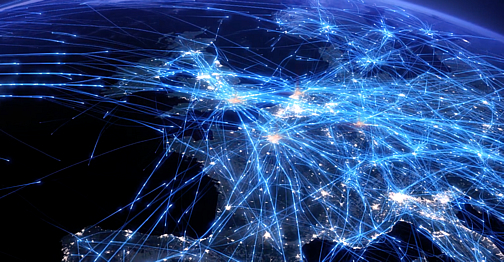
\includegraphics[width=\textwidth]{images/flight-paths}}
				\caption{Air traffic data visualisation. \protect\footnotemark}
				\label{fig:flight_paths}
			\end{figure}

			\footnotetext{\bibentry{nats2014air}}
			
			The format of the data needed to be confirmed before generating it. To do this, a test runner was created to evaluate any performance differences in reading and parsing array data as opposed to objects. The results of this test, which are demonstrated in Figure~\ref{fig:performance_test}, conclude that reading and parsing array data is far more efficient.
			
			\begin{figure}[H]
        		\href{http://jsperf.com/object-and-array-reading}{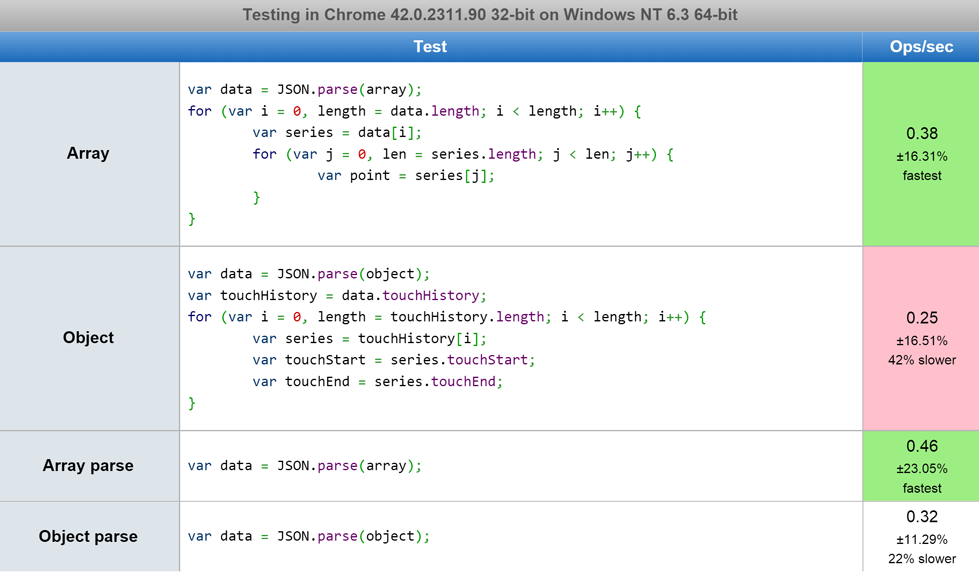
\includegraphics[width=\textwidth,height=8.5cm]{images/performance-test}}
				\caption{The results of the performance test.}
				\label{fig:performance_test}
			\end{figure}
			
			Lines are incredibly difficult to draw in WebGL \footnote{\bibentry{deslauriers2015lines}} and was the first challenge when attempting to develop this visualisation. There are two main methods of rendering a line using the Three.js library: 
			
			\begin{description}
				\item[Line Object:] The default thickness of the line is too thin to highlight intersections with alpha blending. To resolve this, the \emph{lineWidth} property should be used. However, it is not supported in Windows which limits the availability of the system.
				\item[TubeGeometry:] This geometry does not render acute angles accurately and results in a thinner and deformed tube structure. It also does not shade intersecting tubes correctly, which is highlighted in Figure~\ref{fig:tube_geometry}. While the code could be modified through a pull request, this would be too time consuming as the mathematics behind it is very complex and would need to be learned.
			\end{description}
			
			\begin{figure}[H]
        		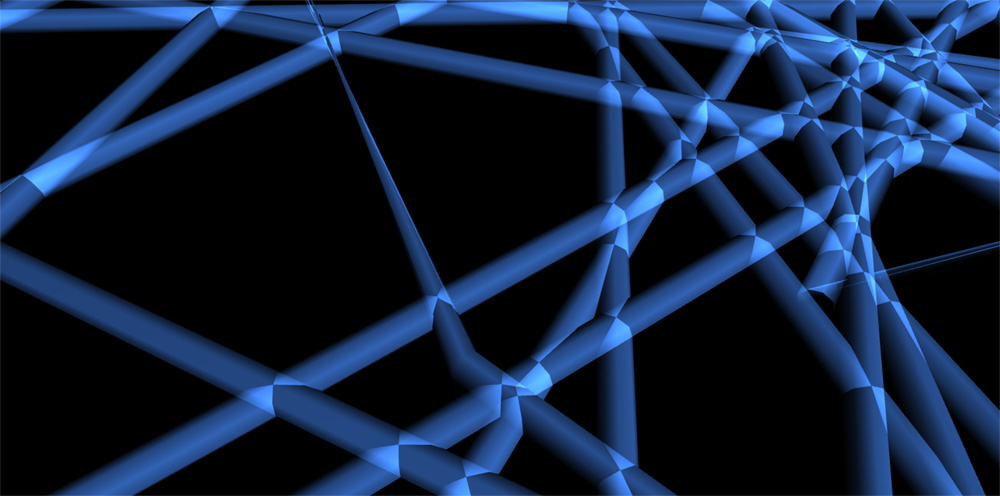
\includegraphics[width=\textwidth]{images/tube-geometry}
				\caption{The issues with TubeGeometry.}
				\label{fig:tube_geometry}
			\end{figure}
			
			The visualisation did provide relatively good results which have been presented in Figure~\ref{fig:proof_of_concept}. However, when closely inspected the issues with its finer details were too prominent. Given the difficulty of amending the issues that arise when rendering a line, this idea was scrapped.
			
			\begin{figure}[H]
        		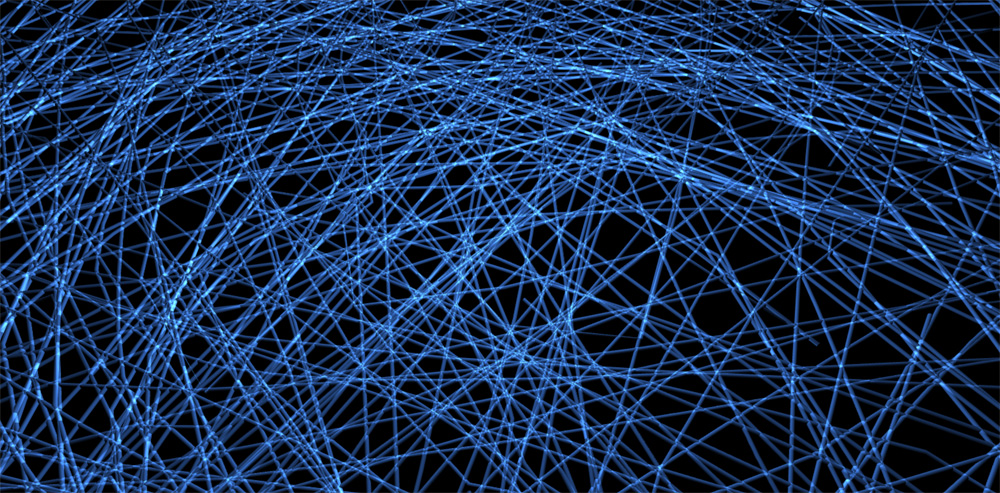
\includegraphics[width=\textwidth]{images/proof-of-concept}
				\caption{An example of the visualisation that was developed.}
				\label{fig:proof_of_concept}
			\end{figure}
		
		}
		
		\newpage
	
		\section{Examples} {
		\label{app:examples}
		
			\subsection{WebGL Globe} {
			\label{app:globe}
		
				\begin{figure}[H]
        			\href{https://www.chromeexperiments.com/globe}{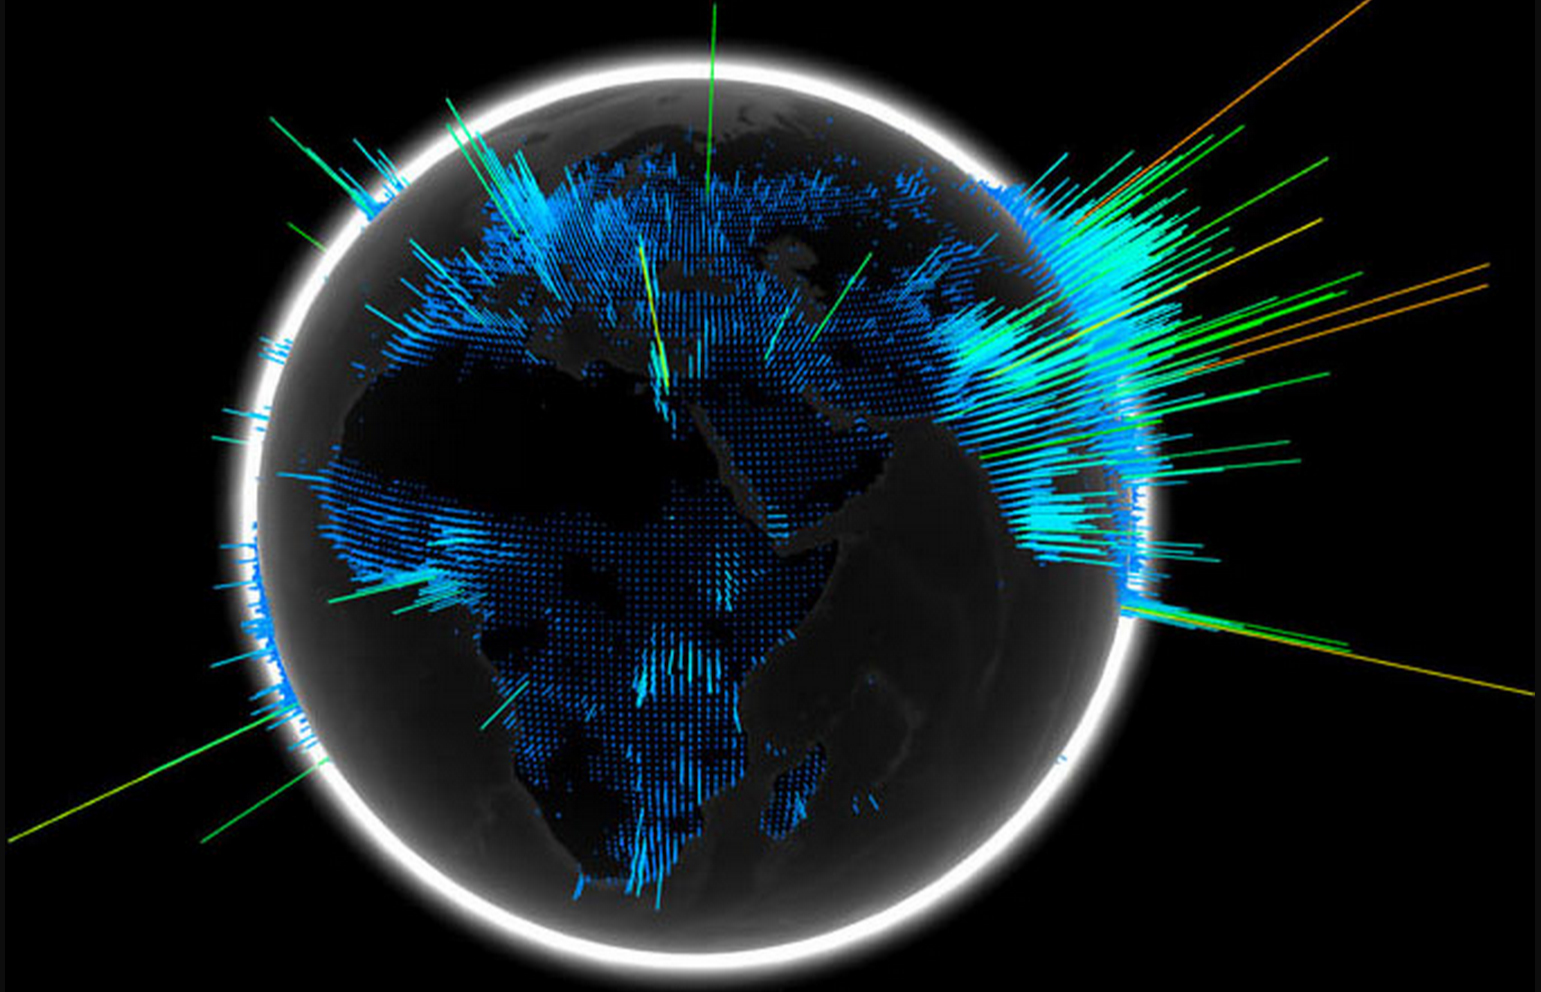
\includegraphics[width=\textwidth]{images/globe}}
					\caption{A screenshot of the WebGL Globe representing population data. \protect\footnotemark}
					\label{fig:webgl_globe}
				\end{figure}

				\footnotetext{\bibentry{google2011globe}}
		
			}
		
			\subsection{NURBS curve and surface} {
			\label{app:nurbs}		
		
				\begin{figure}[H]
        			\href{http://threejs.org/examples/webgl_geometry_nurbs.html}{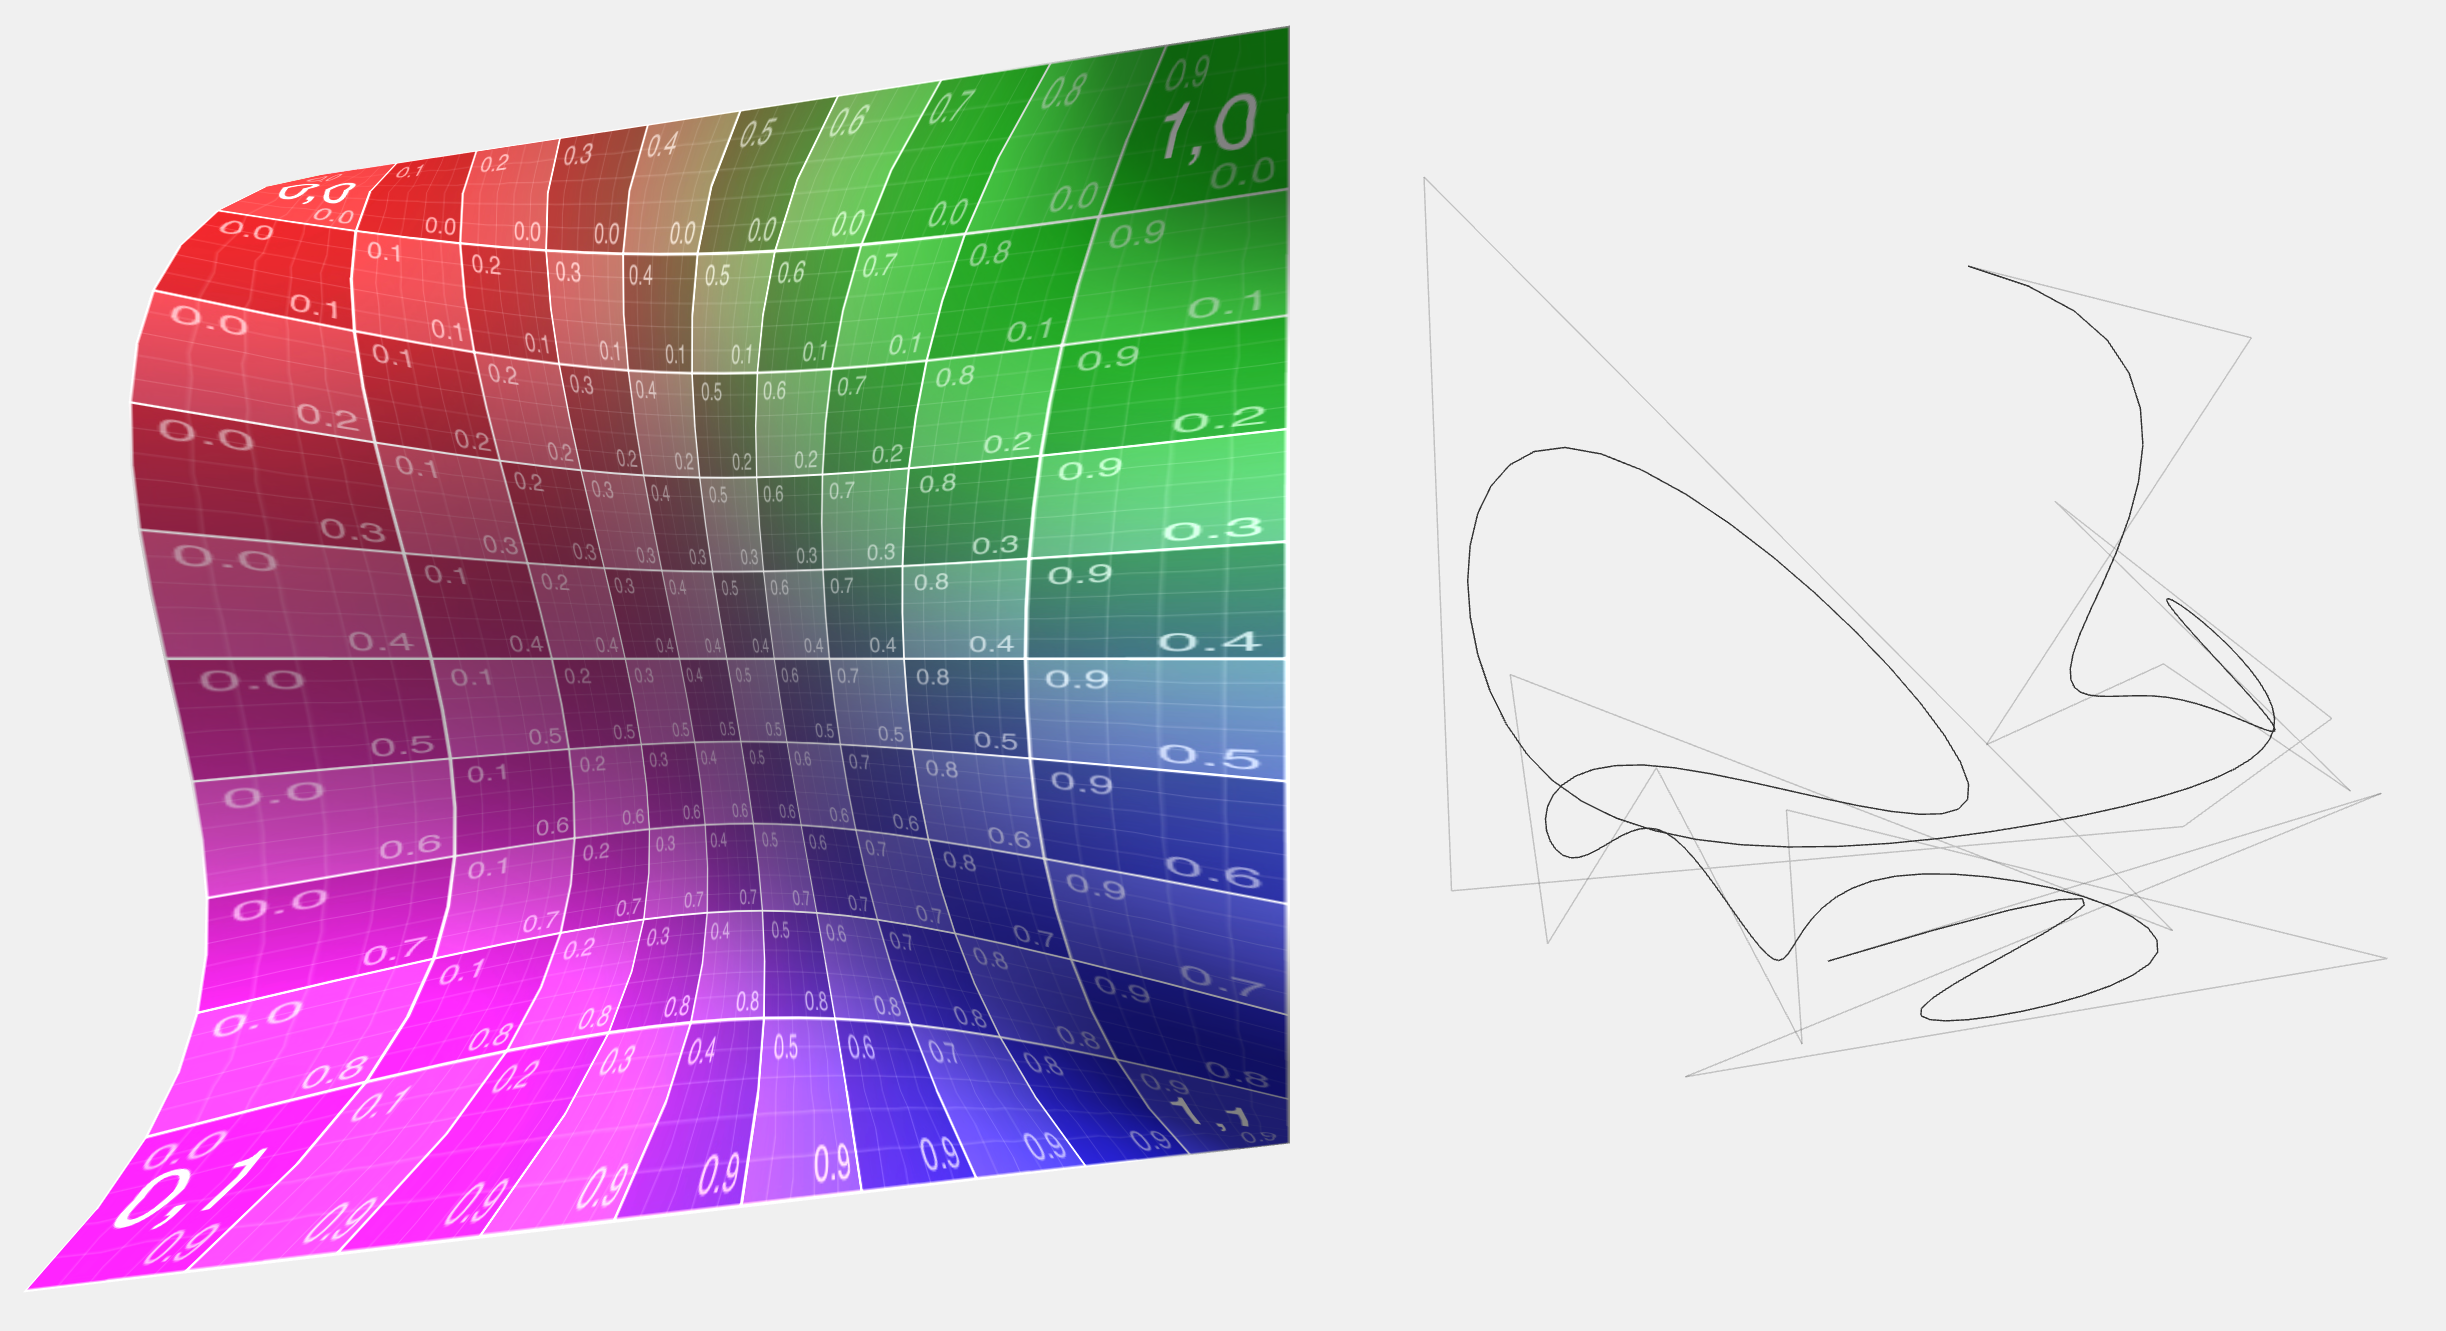
\includegraphics[width=\textwidth,height=8cm]{images/nurbs}}
					\caption{A screenshot of the NURBS curve and surface example.}
					\label{fig:nurbs}
				\end{figure}
		
			}
			
		}
		
		\newpage
		
		\section{Risk assessment} {
		\label{app:risk_assessment}
		
			\subsection{Category legend} {
			\label{app:category_legend}
			
				\begin{table}[H]
				\caption{A list of the categories used in the risk assessment.}
				\begin{tabularx}{\textwidth}{@{}lX@{}}
					\toprule
					\textbf{Risk category} & \textbf{Examples} \\
					\midrule
					Project management & Operational, organisational and contractual software development parameters. \\
					Process management & Planning, staffing, tracking, quality assurance and configuration management. \\
					Technical process & Analysis, design, programming and testing. \\
					Technical product & Requirements stability, design performance, code complexity and test specifications. \\
					\bottomrule
				\end{tabularx}
				\end{table}
			
			}
			
			\subsection{Strategy legend} {
			\label{app:strategy_legend}

				\begin{table}[H]
				\caption{A list of the risk strategies used in the risk assessment.}
				\begin{tabularx}{\textwidth}{@{}lX@{}}
					\toprule
					\textbf{Risk strategy} & \textbf{Description} \\
					\midrule
					Acceptance & The risk is acceptable and will be account for. \\
					Avoidance & An activity will not be performed if it may result in a risk. \\
					Reduction & The severity of the impact or the likelihood of the risk will be reduced. \\
					Research & The risk will be investigated so it can be managed. \\
					Transfer & The risk is shifted to or outsourced to another person, group or organisation. \\
					\bottomrule
				\end{tabularx}
				\end{table}

			}

			\subsection{Risk rating legend} {
			\label{app:risk_rating_legend}

				\begin{table}[H]
				\caption{The mapping between the priority score and its associated risk rating.}
				\begin{tabularx}{\textwidth}{@{}XX@{}}
					\toprule
					\textbf{Priority score} & \textbf{Risk rating} \\
					\midrule
					0 - 19 & Very low \\
					20 - 39 & Low \\
					40 - 59 & Medium \\
					60 - 79 & High \\
					80 - 100 & Very high \\
					\bottomrule
				\end{tabularx}
				\end{table}

			}
			
			\subsection{Risk details} {
			\label{app:risk_details}
			
				\begin{table}[H]
				\caption{The details of the risks that were outlined in Section~\ref{sec:risks}.}
				\begin{spreadtab}{{tabularx}{\textwidth}{@{}llXXXX@{}}}
					\toprule
					@\textbf{Id} & @\textbf{Category} & @\textbf{Likelhood} & @\textbf{Impact} & @\textbf{Score} & @\textbf{Rating} \\
					\midrule
					1 & @Project management & :={35}\% & 95 & (c2 / 100) * d2 & \rating{:={e2 * 100}} \\
					2 & @Technical product & :={10}\% & 80 & (c3 / 100) * d3 & \rating{:={e3 * 100}} \\
					3 & @Technical product & :={10}\% & 100 & (c4 / 100) * d4 & \rating{:={e4 * 100}} \\
					4 & @Process management & :={5}\% & 85 & (c5 / 100) * d5 & \rating{:={e5 * 100}} \\
					5 & @Technical process & :={1}\% & 75 & (c6 / 100) * d6 & \rating{:={e6 * 100}} \\
					6 & @Technical product & :={20}\% & 85 & (c7 / 100) * d7 & \rating{:={e7 * 100}} \\
					7 & @Technical product & :={20}\% & 85 & (c8 / 100) * d8 & \rating{:={e8 * 100}} \\
					\bottomrule
				\end{spreadtab}
				\end{table}
			
			}
		
		}
		
	\end{appendices}
	
\end{document}
